% vim: set spelllang=fr foldmethod=marker:
\lettrineh{P}{uisque} les travaux présentés dans cette thèse portent sur les \rcsfs, il semble indispensable d'introduire tout d'abord les caractéristiques de ces capteurs et des réseaux qu'ils peuvent former.
Le présent chapitre décrit donc le fonctionnement basique des capteurs, des réseaux, et fournit des exemples d'applications.
Dans un second temps, ce sont certains des principaux problèmes soulevés par le déploiement des capteurs qui seront brièvement introduits, notamment la nécessité d'adapter les protocoles employés aux capacités des capteurs, les besoins éventuels de partition du réseau pour en obtenir une gestion plus efficace, ou encore des problèmes de mobilité, de sureté, de sécurité, de résilience.

\section{Réseaux de capteurs sans fil}

    \subsection{De quoi s'agit-il?}
%{{{1
%{{{2
\begin{figure}[!ht]
    \centering
    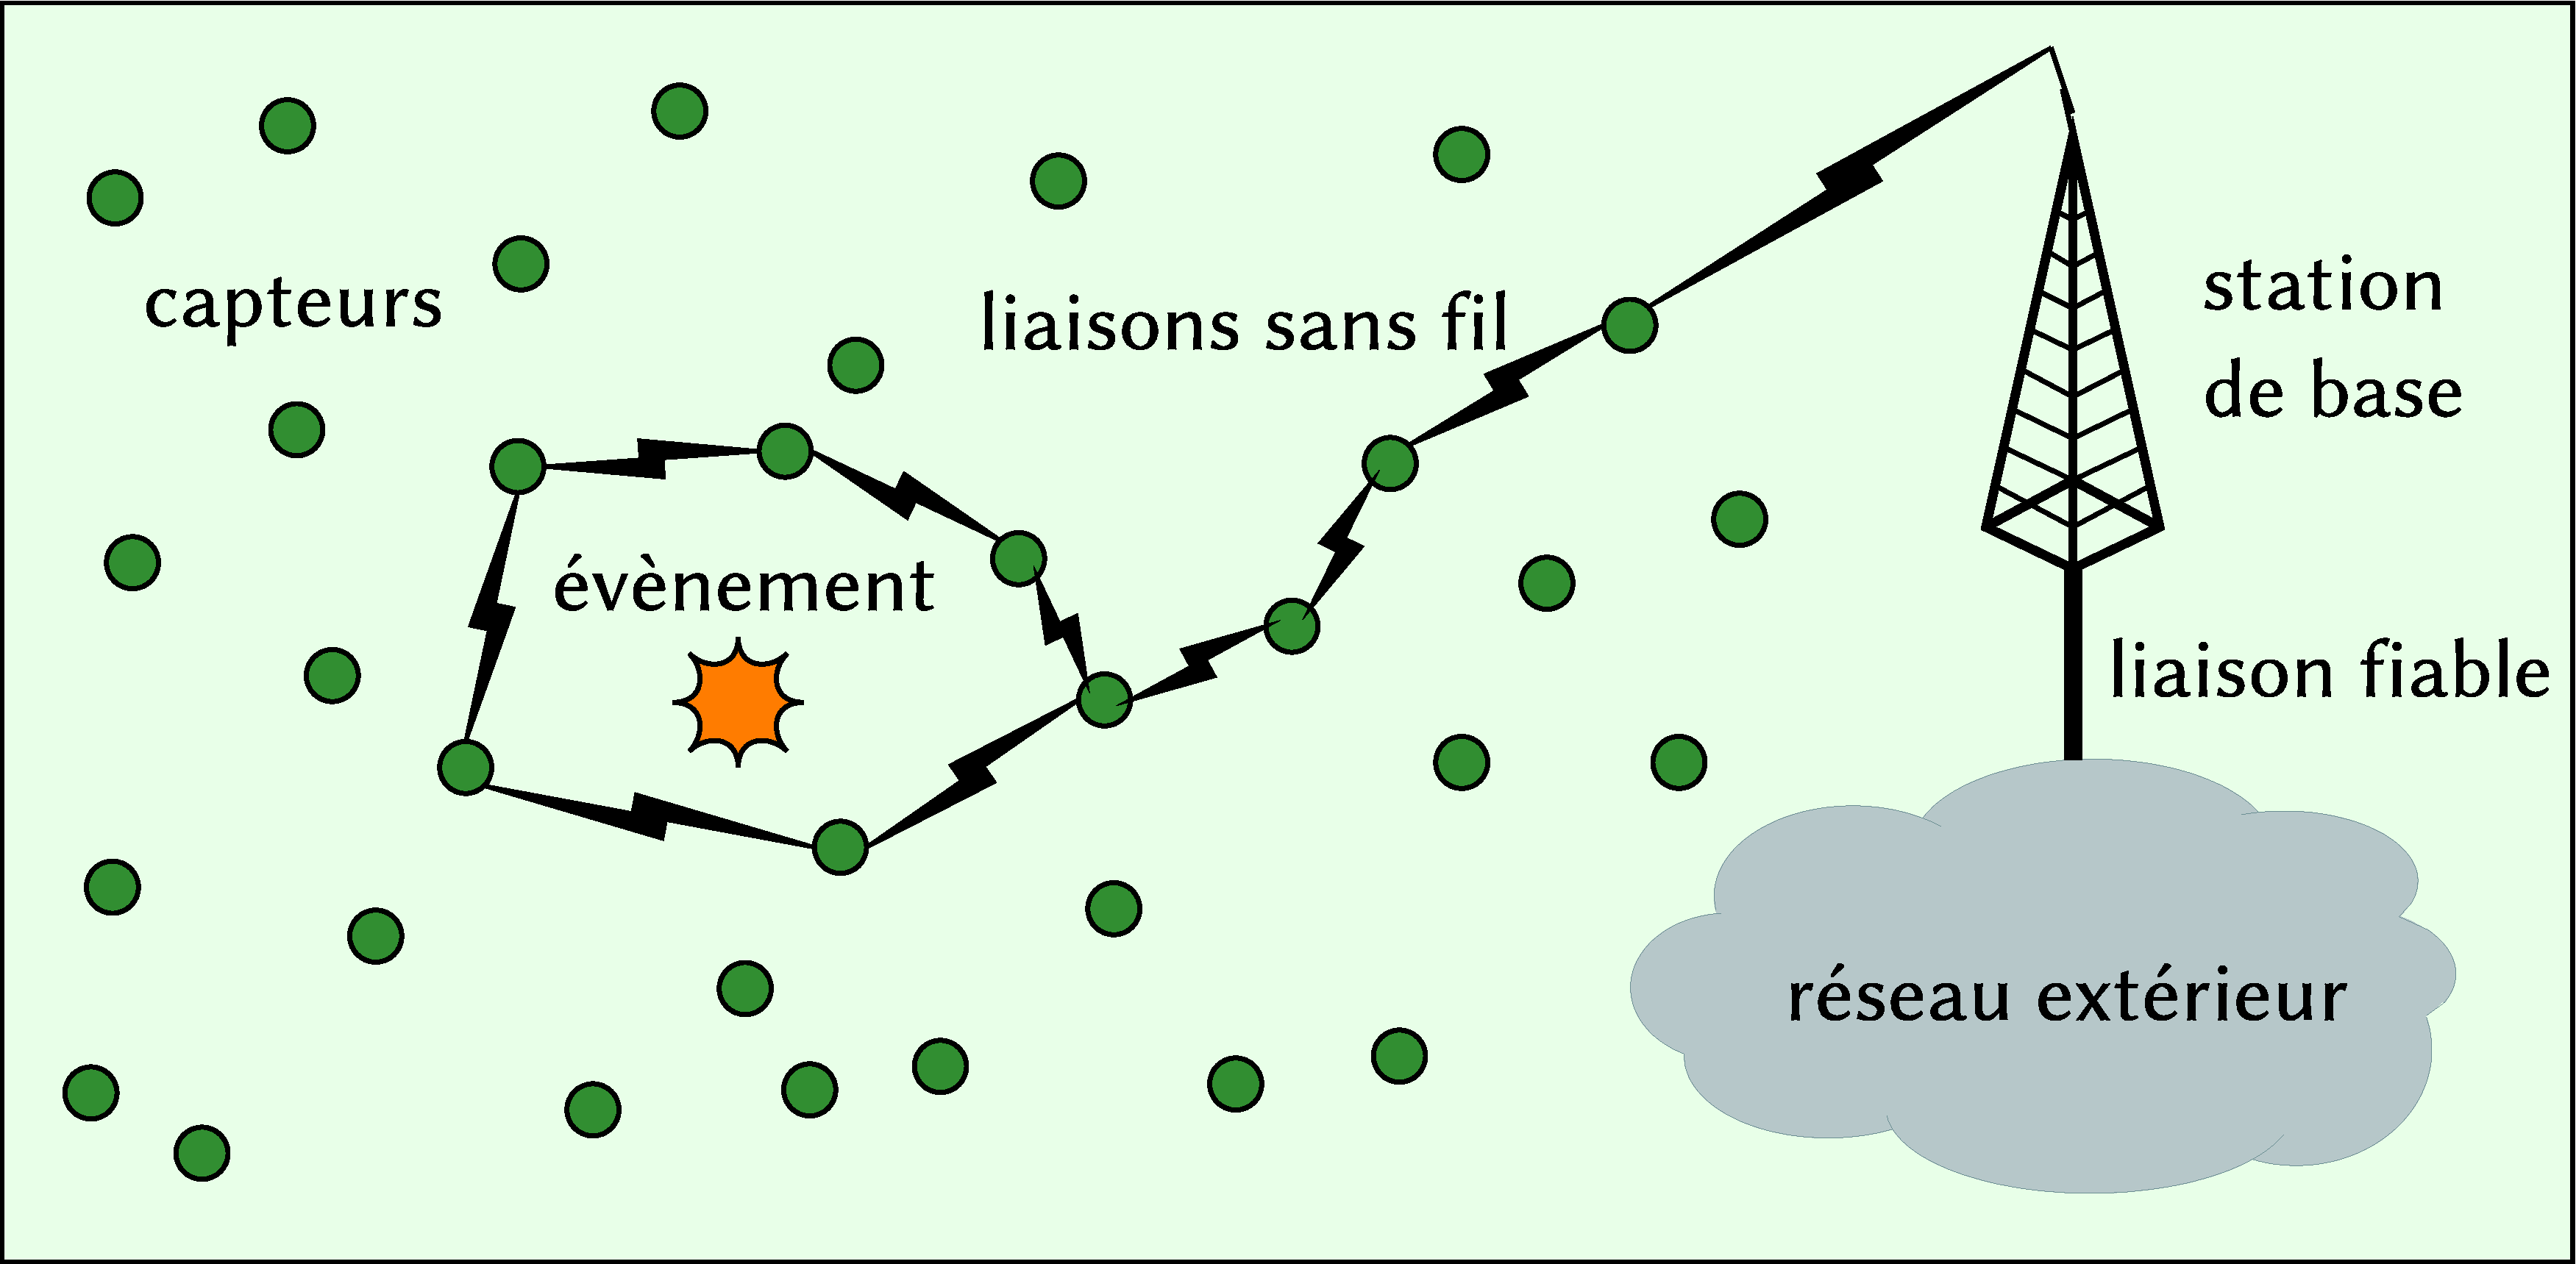
\includegraphics[width=.8\textwidth]{\chapterpath/Figures/WSN_archi.pdf}
    \caption{Schéma simple d'un \rcsf}\label{st:fig:wsnintro}
\end{figure}
Les \rcsfs, ou \textit{\WSN} (pour \wsns en anglais), sont des réseaux constitués de petits appareils, les capteurs, ainsi que d'une \sdb.
\nomenclature{WSN}{\wsns}
Les capteurs échangent par communications hertziennes, en utilisant des protocoles tels ceux définis dans la pile \ieeee.
Le routage des paquets dans le réseau peut faire appel à l'un des nombreux protocoles développés à cet effet (par exemple: \aodv, \olsr), qu'il repose sur un algorithme centralisé (dirigé par une seule entité) ou distribué (exécuté par chaque entité du réseau).
Les capteurs collectent des informations sur leur environnement et les font remonter à la \sdb.
Cette \sdb, ou \BS (pour \bs), ou encore parfois \textit{puits} (\textit{sink} en anglais), est chargée de récolter et traiter les données provenant des capteurs.
Une fois les capteurs déployés, l'administrateur n'interagit plus avec le réseau que par le biais de la \sdb.
Un schéma basique de \rcsf est présenté en \figref{st:fig:wsnintro}
\nomenclature{BS}{\bs}

Il est rare que tous les capteurs d'un \WSN soit directement connectés les uns aux autres.
À la topologie d'un réseau donné est donc très souvent associé le graphe de connectivité du réseau.
Pour cette raison, il est souvent fait référence aux capteurs sous le terme de \textit{nœuds} (ou de \textit{nodes} en anglais).

\begin{figure}[H]
    \centering
    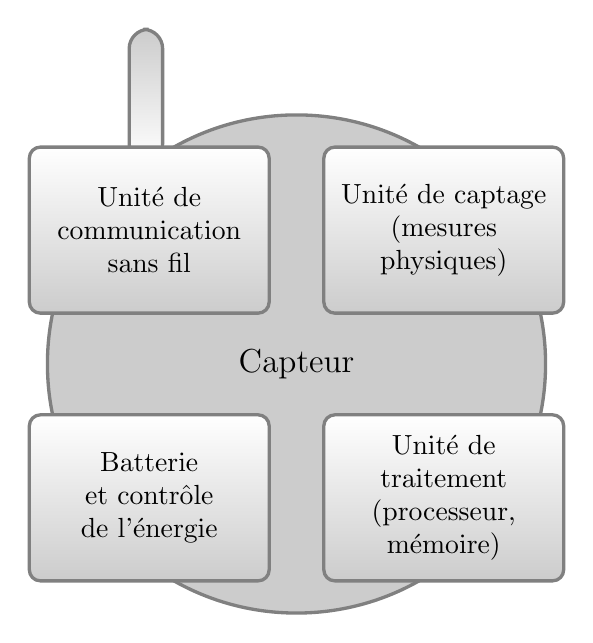
\begin{tikzpicture}[%
        scale=.85,
        sensor/.style={%
            circle,%
            minimum size=18em,%
            very thick,%
            draw=black!50, %
            fill=black!20%
        },%
        module/.style={%
            rounded corners,%
            text width=8em,%
            minimum height=6em,%
            align=center,%
            very thick,%
            draw=black!50, %
            top color=white,%
            bottom color=black!20%
        }%
    ]
    \node (sensor) at (   0, 0) [sensor]{\large Capteur};
    \draw [rounded corners=7pt,top color=black!20,draw=black!50,very thick] (-2,3)--(-2,5)--(-2.5,5)--(-2.5,3)--cycle ;
    \node (mesure) at ( 2.2, 2) [module]{Unit\'e de captage\\(mesures physiques)};
    \node (mesure) at (-2.2, 2) [module]{Unit\'e de\\communication sans fil};
    \node (mesure) at ( 2.2,-2) [module]{Unit\'e de traitement\\(processeur, m\'emoire)};
    \node (mesure) at (-2.2,-2) [module]{Batterie\\et contr\^ole de l'\'energie};
    \end{tikzpicture}
    \caption{Schéma représentant les principaux modules d'un capteur standard}\label{st:fig:sensor}
\end{figure}
Un capteur seul peut être vu comme l'assemblage de quatre modules principaux, représentés en \figref{st:fig:sensor}.
Il s'agit:
\begin{itemize}
    \item d'une unité de captage, chargée de réaliser des mesures physiques (analogiques) sur l'environnement, puis de les convertir en un signal numérique;
    \item d'un module de traitement, composé principalement d'un processeur et de mémoire (mémoire vive et mémoire non volatile), qui assure le fonctionnement du système d'exploitation, gère les interactions entre les différents modules, et surtout traite les données récoltées;
    \item d'une unité de transmission/réception utilisée pour les communications hertziennes;
    \item d'une batterie, accompagnée d'une unité de contrôle de l'énergie elle-même chargée d'alimenter de façon efficace les autres modules du capteur.
\end{itemize}
%2}}}
%1}}}

    \subsection{Applications}
%{{{1
Le champ d'application des \WSN est très vaste, et n'a de cesse de s'élargir au fil du temps et des avancées technologiques.
Toutes ne font pas l'objet de publications scientifiques, mais certaines sont régulièrement évoquées en tant qu'exemples, ou bien font l'actualité dans le domaine des nouvelles technologies voire le domaine commercial.

        \paragraph{Applications environnementales}
%{{{2
La gestion de l'environnement par l'Homme a de plus en plus recours à des mesures distribuées reposant sur l'usage de capteurs.
Les prévisions météorologiques (reposant sur des mesures d'hygrométrie, de pression de l'air, \etc) ont été l'un des premiers champs d'application des capteurs.
Les mesures de qualité de l'air et de taux de pollution, en ville comme en campagne, se généralisent peu à peu.
Les réseaux de capteurs permettent même de pousser la mesure de ce taux vers de nouveaux milieux, comme les glaciers~\cite{MPROH05} ou bien les océans.

L'agriculture est également susceptible d'avoir recours aux capteurs: des essais sont menés sur la réalisation de mesures faites par des microcapteurs semés en même temps que les cultures, permettant de surveiller au mieux les conditions de développement de ces dernières.
Placés judicieusement dans l'habitat naturel de certaines espèces, les capteurs peuvent être utilisés pour suivre et analyser le comportement de la faune d'un milieu~\cite{KDA14}.

En forêt, les \rcs peuvent permettre de détecter les départs de feu et de lutter plus efficacement contre les incendies.
Et en zones à risques, ils peuvent être utilisés pour mesurer l'activité sismique ou volcanique du sol, et permettre une meilleure anticipation des phénomènes naturels.
L'industrie a également recours à ces réseaux pour détecter d'éventuelles fuites de produits toxiques (pétrole, gaz, éléments radioactifs).

Il est à noter que certaines de ces applications touchent à des domaines critiques (en termes de sécurité des installations, voire de vies humaines): il est indispensable d'assurer le bon fonctionnement du réseau déployé dans un tel contexte.
%2}}}

        \paragraph{Surveillance et détection}
%{{{2
Les \rcsfs sont aussi employés pour des mesures de sureté ou de sécurité, par exemple pour surveiller l'intégrité structurelle de certaines architectures (ferroviaires, aérospatiales, maritimes, ou plus simplement dans le bâtiment: gros œuvre, ouvrages d'art) et peuvent permettre une prévention efficace des pannes matérielles~\cite{SCOA13}.
Mis à part la détection de pannes, les capteurs peuvent être utilisés dans des systèmes de vidéosurveillance en milieu urbain, ou sur des sites sensibles afin de prévenir les intrusions humaines, ou bien pour détecter des incidents ou encore établir le suivi de certaines entités; la gestion du trafic routier, ou même seulement des autobus, en sont des exemples.
Le CEREMA (Centre d'études et d'expertise sur les risques, l'environnement, la mobilité et l'aménagement) a mis en ligne un site Internet particulièrement riche en exemples d'application des capteurs, et détaillant notamment les différentes technologies utilisées pour réaliser les mesures~\cite{sti}.
Pour exemple la seule détection de véhicules sur les voies de circulation peut reposer sur:
\begin{itemize}
    \item la détection d'une modification du champ magnétique environnant;
    \item la pression exercée par le véhicule sur la voie;
    \item la variation de la pression dans un tube pneumatique;
    \item les déformations de la structure d'un pont sous le poids des véhicules;
    \item les variations d'intensité lumineuse ou sonore;
    \item le renvoi d'ondes radar, ou lumineuses (laser), ou infrarouges, ou ultrasons;
    \item l'analyse d'image vidéo visibles ou infrarouges, par reconnaissance de forme, ou bien par détection du mouvement des groupes de pixels…
\end{itemize}
\nomenclature{laser}{\textit{Light Amplification by Stimulated Emission of Radiation}}
\nomenclature{radar}{\textit{RAdio Detection And Ranging}}
%2}}}

        \paragraph{Domaine militaire}
%{{{2
La surveillance et la détection sont aussi très utilisés dans le domaine militaire.
Qu'il s'agisse de mener des opérations de renseignement ou bien de suivre l'évolution d'un combat sur le champ de bataille, pour analyser les cibles, relier entre eux fantassins et véhicules de tous types, pour détecter les agents radioactifs, chimiques ou biologiques répandus par un ennemi, toutes les informations sont bonnes à prendre~\cite{ASSC02}.
Un maximum d'entre elles doivent être remontées au centre de commandement, afin de permettre une supervision optimale des forces en mouvement.
Plus encore que les exemples précédents, l'usage des capteurs en contexte militaire implique de fortes contraintes en termes de \secu pour le réseau déployé.
%2}}}

        \paragraph{Médecine}
%{{{2
Certains usages des capteurs tiennent du domaine médical~\cite{SZFDXC14}.
Il peut s'agir par exemple de faire communiquer un ou plusieurs implants avec un contrôleur externe.
Il peut également être question d'employer des microcapteurs pour analyser avec précisions des variables corporelles (taux de glycémie, surveillance des organes vitaux) ou bien, sur une plus courte durée, pour traiter avec précision une pathologie locale (des cellules cancéreuses par exemple).
%2}}}

        \paragraph{Grand public}
%{{{2
Le public a lui aussi de plus en plus accès à des applications reposant sur les capteurs.
En domotique par exemple, la température des différentes pièces d'un lieu d'habitation peut être rendue accessible à tout instant, tandis que des fonctions comme l'activation de volets électriques, l'ouverture de portes, l'activation de sources lumineuses ou de dispositifs de chauffage peuvent être effectuées à distance par l'habitant (par exemple par le biais d'une application logicielle sur téléphone portable) ou bien de façon automatique en fonction des besoins identifiés à partir des données récoltées~\cite{ASSC02}.

Un autre domaine d'application en voie de développement est ce que l'on appelle l'\textit{\idx{Internet des objets}} (\textit{the Internet of things} en anglais), et qui consiste en quelque sorte à étendre \idx{Internet} au monde réel, par le biais d'une interconnexion réseau entre les objets de la vie courante: de plus en plus d'objets du quotidien tendent à devenir «connectés».
Ils se voient alors équipés de capteurs, d'un module de communication sans fil, et offrent de nouvelles possibilités en termes d'usages.
Quelques exemples:
\begin{itemize}
    \item les montres (interfacées avec les téléphones «intelligents» pour afficher des notifications diverses);
    \item les ampoules d'éclairage (gestion de la luminosité, de la couleur de l'éclairage, parfois dynamiques);
    \item les ceintures (accessoires vestimentaires: réajustement automatique du réglage, collecte de données sur le tour de taille pour le contrôle du poids);
    \item les réfrigérateurs (gestion des réserves alimentaires, création de listes d'achat);
    \item les véhicules autonomes, tels que les voitures sans conducteurs ou les drones (pilotage de l'engin, relevé de mesures tactiques pour les drones militaires).
\end{itemize}
Des puces RFID (de l'anglais \textit{Radio Frequency Identification}, «identification sur fréquences radio») se retrouvent par ailleurs de plus en plus utilisées, entre autres raisons pour faciliter de telles interactions dans le monde «connecté»~\cite{TW10}.
Au fur et à mesure que ces objets intègrent la vie quotidienne des utilisateurs, ils auront probablement tendance à communiquer de plus en plus entre eux, entre objets, en ne centralisant les données que sur une seule interface présentée à l'utilisateur final.
\nomenclature{RFID}{\textit{Radio Frequency IDentification}}
%2}}}

        \paragraph{}
Les applications présentées ici ne représentent bien sûr que quelques exemples parmi les nombreux usages existants des capteurs~\cite{ASSC02}, dont la quantité ne cesse par ailleurs de croitre au fil du temps.
%1}}}

    \subsection{Contraintes en ressources}
%{{{1
De par leur petite taille, et à cause de leurs déploiement dans des zones souvent difficiles d'accès, les capteurs n'embarquent qu'une quantité limitée de matériel, qui ne peut pas toujours être remplacé.
Les capteurs se retrouvent donc avec des capacités limitées~\cite{BMS13}, notamment en ce qui concerne:
\begin{itemize}
    \item les \textbf{capacités de calcul}: les processeurs embarqués sont relativement peu puissants, principalement pour des raisons de cout.
        Les algorithmes exécutés par les capteurs doivent donc être de complexité relativement basse;
    \item les \textbf{capacités de mémoire}: les capteurs disposent de mémoire vive (RAM, \textit{Random Access Memory}, «mémoire à accès non séquentiel» en anglais) et d'un peu d'espace de stockage, mais ils ne sont pas du tout conçus pour sauvegarder de grandes bases de données.\nomenclature{RAM}{\textit{Random Access Memory}}
        Les informations récoltées doivent être acheminées à la \sdb, et non stockées sur le long terme par les capteurs eux-mêmes;
    \item l'\textbf{énergie disponible}: les capteurs disposent d'une batterie qui leur fournit une quantité d'énergie finie, et (la plupart du temps) non rechargeable.
        Il est donc essentiel de conserver à l'esprit une gestion parcimonieuse de l'énergie pour tout programme implémenté sur les capteurs.
        Des calculs importants, ainsi que des émissions/réceptions d'ondes électromagnétiques nombreuses ou mal gérées, sont les principaux facteurs d'un épuisement prématuré de la batterie.
\end{itemize}

Il est à noter qu'au regard de ces contraintes qui affectent les capteurs, la \sdb est considérée comme disposant de capacités «illimitées».
%1}}}

    \subsection{Communications sans fil}
%{{{1
%{{{2
Comme l'indique leur nom, les \rcsfs n'utilisent aucun câble physique pour communiquer entre eux ou avec la \sdb: toutes les transmissions sont effectuées par voie hertzienne.
Chaque capteur est équipé d'un module radio utilisé alternativement pour émettre et pour recevoir.
La plupart du temps ces modules sont capables de changer de fréquence de communication, ainsi que de moduler la puissance d'émission utilisée pour les transmissions.

Les protocoles de communication déployés sur cette architecture sont multiples (on parle d'\textit{encapsulation} des données).
Il faut pouvoir communiquer de pair à pair entre nœuds voisins, tout comme il faut être capable de faire parvenir un message à un nœud éloigner en faisant retransmettre les paquets par des nœuds relais successifs, d'assurer certains services comme le maintien de session, ou de gérer des applications.
Comme dans la plupart des réseaux informatiques, l'empilement des protocoles reprend donc le modèle \tcpip~\cite{TW10} (schéma concret lui-même issu du modèle théorique \idx{OSI}, de l'anglais \textit{Open Systems Interconnection}), présenté en \figref{st:fig:tcpip}.
\nomenclature{OSI}{\textit{Open Systems Interconnection}}
\begin{figure}[H]
    \centering
    \begin{tabular}{c |c| l}
        \multicolumn{2}{c}{} & Exemples:\\
        \cline{2-2}
        5 & Application & HTTP, FTP, SSH\\
        \cline{2-2}
        4 & Transport   & TCP, UDP\\
        \cline{2-2}
        3 & Réseau      & IP\\
        \cline{2-2}
        2 & Liaison     & \ieeee (\csmaca)\\
        \cline{2-2}
        1 & Physique    & ondes électromagnétiques\\
        \cline{2-2}
     \end{tabular}
    \medskip
    \caption{Modèle TCP/IP}\label{st:fig:tcpip}
\end{figure}
\nomenclature{TCP}{\textit{Transmission Control Protocol}}
\nomenclature{IP}{\textit{Internet Protocol}}
\nomenclature{UDP}{\textit{User Datagram Protocol}}
\nomenclature{HTTP}{\textit{HyperText Transfer Protocol}}
\nomenclature{FTP}{\textit{File Transfer Protocol}}
\nomenclature{SSH}{\textit{Secure SHell}}

Certains standards normalisés définissent l'usage de protocoles spécifiques sur les trois premières couches.
Les principaux standards qui sont employés dans les \rcs sont les piles \ieeee (correspondant à la marque \wifi) et \ieeeff (sur laquelle sont basée la marque \zigbee et le standard \ietf \slowpan), et dans une moindre mesure la pile \ieeefo (correspondant à la marque \bluetooth).
\nomenclature{IETF}{\textit{Internet Engineering Task Force}}
\nomenclature{IEEE}{\textit{Institute of Electrical and Electronics Engineers}}
\nomenclature{6LoWPAN}{\textit{IPv6 over Low power Wireless Personal Area Networks}}
%2}}}

            \paragraph{La couche physique}
%{{{2
Cette couche concerne l'émission et la réception en soi des ondes électromagnétiques, et l'encodage utilisé pour leur faire porter des valeurs numériques (par opposition à un signal analogique)~\cite{TW10}
Les réseaux sans fil ont la particularité de ne pas pouvoir restreindre l'envoi d'un paquet vers son seul destinataire: un paquet émis par transmission électromagnétique est reçu par tout nœud voisin (\cad à distance suffisamment faible pour être couvert par la portée d'émission de l'émetteur) qui écoute le canal (donc les plages de fréquences concernées) au moment de la transmission.
Il est parfois possible de se servir d'une \idx{antenne directionnelle} pour réduire sensiblement les directions dans laquelle est réalisée la diffusion et pour augmenter le ratio de la puissance du signal émis sur l'énergie consommée par l'envoi; mais cet équipement couteux n'est que très rarement utilisé dans les réseaux de capteurs.

Une propriété fréquemment employée en revanche est la capacité à moduler la puissance du signal en fonction des besoins.
Plus le signal est fort, plus il portera loin (et permettra d'atteindre des nœuds distants).
Naturellement, l'émission consommera également plus d'énergie
%2}}}

            \paragraph{La couche de liaison de données}\label{st:ssec:mac}
%{{{2
La deuxième couche du modèle fournit les moyens fonctionnels et procéduraux pour le transfert des données entre deux entités du réseau~\cite{TW10}.
Elle permet aussi, le plus souvent, de détecter et éventuellement corriger certaines erreurs survenues sur la couche physique (en cas de perturbation ou dégradation du signal électromagnétique).
Elle se décompose en deux sous-couches: la couche de contrôle de la liaison logique (\llc, pour \textit{Logical Link Control} en anglais, «contrôle de la liaison logique») et la couche du contrôle d'accès au support (\mac, pour \textit{Media Access Control}, «contrôle d'accès au support»).
\llc est la sous-couche haute, utilisée pour fiabiliser la sous-couche \mac, intervient peu dans les \rcs.
Le protocole de couche \mac définit la manière dont les différents agents du réseau accèdent au médium de transmission de façon à limiter les collisions, et à garantir un accès le plus souvent équivalent au médium pour tous les nœuds.
\begin{table}[!ht]
    \caption{Méthodes d'accès au médium de transmission}\label{st:tab:mac}
    \centering
    \medskip
    \begin{small}
        \begin{tabular}{m{.2\textwidth}|m{.2\textwidth}|m{.48\textwidth}}
            \toprule
            \textsc{Nom anglais} & \textsc{Traduction} & \textsc{Description}\\
            \midrule
            \multicolumn{3}{c}{Commutation de circuits et création de canaux}\\
            \midrule
            \textit{Frequency Division Multiple Access} (\fdma) & Accès multiple par répartition en fréquence & Plusieurs canaux basés sur des fréquences différentes\\
            \midrule
            \textit{Code division multiple access} (\cdma) & Accès multiple par répartition en code & Étalement du spectre de fréquence\index{etalement@étalement de spectre} utilisé en conjonction avec techniques comme les sauts de fréquences ou la génération de bruit pseudo-aléatoires (avec la même séquence pseudo-aléatoire appliquée au signal côté émetteur comme côté destinataire)\\
            \midrule
            \textit{Time division multiple access} (\tdma) & Accès multiple à répartition dans le temps & Un seul canal dont l'accès est réparti par créneaux dans le temps\\
            \midrule
            \textit{Space division multiple access} (\sdma) & Accès multiple à répartition dans l'espace & Plusieurs canaux spatiaux obtenus à l'aide d'antennes directionnelles. À noter: les antennes directionnelles\index{antenne directionnelle} augmentent sensiblement le cout de production des capteurs.\\
            \midrule
            \multicolumn{3}{c}{Mode d'accès par paquet}\\
            \midrule
            \textit{Contention based random multiple access methods} & Accès par contention & Contention par le nœud du paquet à envoyer jusqu'à ce que le protocole le lui autorise. Dans cette catégorie se trouve notamment le protocole \csmaca (\textit{Carrier Sense Multiple Access with Collision Avoidance}, accès multiple par écoute du canal avec esquive de collision), très utilisé dans les réseaux sans fil (\ieeee entre autres).\\
            \midrule
            \textit{Resource reservation (scheduled) packet-mode protocols} & Réservation des ressources & Réservation par un nœud des ressources (par exemple: créneau temporel) nécessaires à la transmission)\\
            \midrule
            \multicolumn{3}{p{.95\textwidth}}{D'autres modes d'accès par paquet (\textit{token passing, polling}) existent mais ne sont pas utilisés dans les \rcs}\\
            \bottomrule
         \end{tabular}
     \end{small}
\end{table}
Les différents modes d'accès au médium existants sont résumés dans la \tabref{st:tab:mac}.
Certains d'entre eux consistent à créer des canaux de transmission distincts, tandis que d'autres déterminent l'accès à une même bande de fréquence en instaurant des règles.
\nomenclature{MAC}{\textit{Media Access Control}}
\nomenclature{LLC}{\textit{Logical Link Control}}
\nomenclature{FDMA}{\textit{Frequency Division Multiple Access}}
\nomenclature{CDMA}{\textit{Code Division Multiple Access}}
\nomenclature{SDMA}{\textit{Space Division Multiple Access}}
\nomenclature{TDMA}{\textit{Time  Division Multiple Access}}
\nomenclature{CSMA}{\textit{Carrier Sense Multiple Access}}
\nomenclature{CSMA/CA}{\textit{Carrier Sense Multiple Access with Collision Avoidance}}

De ces modes d'accès sont dérivés de très nombreux protocoles de couche \mac, dont plusieurs ont été conçus spécifiquement pour les \rcs~\cite{YB09}.
Par exemple, en dehors des standards \ieee, le protocole \smac~\cite{YHE02} fait alterner périodes «actives» et périodes de sommeil aux capteurs afin de préserver leur batterie.
Les capteurs sont associés dans des groupes (qui ne correspondent pas tout à fait à des clusters) dont tous les membres sont en éveil de manière simultanée, afin de pouvoir communiquer à l'aide d'une version modifiée de \csmaca tel que défini dans le standard \ieeee.
\nomenclature{S-MAC}{\textit{Sensor-MAC}}
%2}}}

            \paragraph{La couche réseau}
%{{{2
Cette couche, pour les capteurs sans fil, repose le plus souvent sur le protocole \ip (\textit{Internet Protocol} an anglais), que ce soit en version 4 ou 6 (la version 6 est notamment utilisée avec la pile \slowpan), pour l'adressage, et sur un protocole de routage qui détermine comment les paquets sont retransmis saut après saut dans le réseau~\cite{TW10}.

Les \rcsfs composent en quelque sorte une sous-famille des réseaux sans fil \adhoc (ou \wanet, de l'anglais \textit{wireless Ad hoc Network}), et une grande partie des protocoles et algorithmes utilisés proviennent du monde des \wanet.
Des exemples classiques de ces algorithmes de routage incluent \aodv (\textit{Ad hoc On-Demand Distance Vector Routing})~\cite{aodv} ou son évolution \dsr~\cite{dsr} (\textit{Dynamic Source Routing}), \olsr~\cite{olsr} (\textit{Optimized Link State Routing Protocol}) ou ses évolutions \dsdv (\textit{Destination-Sequenced Distance Vector routing}) et \batman (\textit{Better Approach To Mobile Adhoc Networking}), \etc.
Ces protocoles se répartissent le plus souvent en deux grandes classes: les protocoles «proactifs» reposant sur une table de \idx{routage} établie \apriori, en amont des requêtes (\aodv par exemple); et les protocoles de routage «à la demande» (dont \olsr), qui établissent les routes à la volée lorsqu'une requête de retransmission parvient au nœud relais.
\nomenclature{AODV}{\textit{Ad hoc On-demand Distance Vector routing}}
\nomenclature{DSR}{\textit{Dynamic Source Routing}}
\nomenclature{OLSR}{\textit{Optimized Link State Routing protocol}}
\nomenclature{DSDV}{\textit{Destination-Sequenced Distance Vector routing}}
\nomenclature{B.A.T.M.A.N.}{\textit{Better Approach To Mobile Adhoc Networking}}
\nomenclature{WANET}{\textit{Wireless Ad hoc NETwork}}
%2}}}

            \paragraph{La couche transport}
%{{{2
Cette couche gère les communications de bout en bout entre processus.
Les protocoles les plus fréquemment utilisés, \tcp (\textit{Transmission Control Protocol}) et \udp (\textit{User Datagram Protocol}) assurent l'ordonnancement des paquets et permettent d'éviter les pertes, les doublons et la corruption des paquets~\cite{TW10}.
Le protocole \tcp permet en plus à deux entités de communiquer en mode connecté en établissant une session (début, fin et validation des échanges).
En raison des données de contrôle que ces protocoles impliquent, ils ne sont pas systématiquement implémentés dans les \rcs (ils le sont parfois dans des versions allégées).
%2}}}

            \paragraph{La couche application}
%{{{2
La dernière couche gère les échanges applicatifs entre les différents agents du réseau, et encapsule les données utiles au format désiré pour leur traitement final~\cite{TW10}.
Il s'agit de la couche la plus haut niveau  du modèle.
Elle assure un service propre à l'application déployée, et les protocoles déployés à ce niveau dépendent donc totalement de l'objectif final du réseau, il n'y a donc pas de standard propre aux \rcs.
%2}}}
%1}}}

    \subsection{Terminologie employée}
%{{{1
            \paragraph{Capteurs et nœuds}
%{{{2
Un \rcsf est souvent représenté sous forme de graphe.
En conséquence, il est souvent fait références aux capteurs eux-mêmes sous le terme de «nœuds».
Nous parlerons plutôt de capteurs lorsque nous évoquerons les «\rcs» eux-mêmes, ainsi que les mesures physiques qu'ils réalisent sur leur environnement, et plutôt de nœuds lorsque nous sommes amenés à travailler sur des graphes.
Mais la plupart du temps, ces deux termes peuvent être employés dans cette thèse de manière complètement interchangeable.
Leur alternance n'a le plus souvent que pour but de limiter les répétitions au sein d'une phrase.
%2}}}

            \paragraph{Nœuds normaux}
%{{{2
Les «nœuds normaux» ont deux significations possibles selon le contexte.
\begin{enumerate}
    \item Lorsqu'il est question de partition, de «clusterisation» du réseau, un nœud \textit{normal} est un nœud qui n'a pas été sélectionné pour assurer la fonction de «chef» du cluster, de \ch. De même lorsque des nœuds de contrôle (\cns ou \vns) ont été sélectionné, les nœuds \textit{normaux} sont les nœuds qui n'ont pas été sélectionnés (ni comme nœud de contrôle, ni comme \ch): ils poursuivent donc simplement leur rôle de collecte et de transmission des données mesurées.
    \item Lorsqu'il est question de \secu et d'attaques menées depuis l'intérieur du réseau, un nœud \textit{normal} désigne un nœud non compromis. Les termes «nœud légitime», «nœud sain» ont le même sens dans cette thèse. Ils sont à opposer au nœud «attaquant», «compromis», «corrompu» ou occasionnellement «cupide».
\end{enumerate}
%2}}}

            \paragraph{Attaquant}
%{{{2
Le terme d'«attaquant» fait par principe référence à l'entité consciente qui se trouve à l'origine d'une attaque, qu'il s'agisse d'une personne seule ou d'une organisation.
Il arrive toutefois que par abus de langage, l'«attaquant» soit utilisé en tant que raccourci pour «le nœud attaquant», c'est à dire le nœud corrompu par l'\textit{attaquant} réel, depuis lequel l'attaque est menée au sein du réseau.
%2}}}

            \paragraph{Exploitant}
%{{{2
L'\textit{exploitant} du réseau désigne l'entité (entité humaine ou organisation) qui exploite le \rcsfs: l'entité qui interagit avec la \sdb, de l'«autre côté» du réseau, pour récupérer et analyser les données collectées par les capteurs et remontées jusqu'à elle.
Sauf précision contraire, on fait généralement l'amalgame avec l'\textit{administrateur} du réseau, qui procède directement à sa mise en place et éventuellement à son maintien en fonction.
%2}}}

            \paragraph{Des capteurs conscients!}
%{{{2
Il va de soi qu'un capteur est un appareil dépourvu de vie et de conscience.
Par abus de langage, des raccourcis sont parfois empruntés dans cette thèse et leur prêtent des intentions ainsi qu'une durée de vie.
Ainsi il arrive que les capteurs «cherchent à», «essayent de», «veulent» réaliser des actions; ou bien qu'ils «prétendent» être de meilleurs candidats au poste de \ch.
De même, ils sont susceptibles de «mourir» lorsque leur batterie est épuisée.
Ces tournures, bien qu'abusives en termes d'exactitude du langage, permettent lorsqu'elles sont employées de simplifier les explications.
%2}}}
%1}}}
